\chapter{Appendix}\label{ch:appendix}

\section*{Appendix B: Blackbody Function}

Even at an undergraduate level, we're all fairly familiar with \emph{blackbody radiation}. The easiest way to deduce the expression for the energy density of photons in \emph{thermal equilibrium} (STE) inside a cavity is by the means of statistical mechanics.
\par Remember the Bose-Einstein distribution ($\mu = 0$)
\begin{equation*}
	n = \frac{1}{\exp(h\nu/kT)-1}
\end{equation*}
and the phase space density of states (per unit volume)
\begin{equation*}
	\rho(\nu)\,\text{d}\nu = \frac{4\pi h g \nu^{3}}{c^{3}}\,\text{d}\nu
\end{equation*}
from which deducing the expression from internal energy is straightforward. Remembering $g=2$ is the quantum degeneracy of photons, a simple moltiplication of the previous expressions yields
\begin{equation}
	U_{\nu}\,\text{d}\nu = \frac{8\pi h}{c^{3}}\frac{\nu^{3}}{\exp(h\nu/kT)-1}\,\text{d}\nu
    \label{eq:blackbody_endens}
\end{equation}
\par The energy of a photon is $E_{\gamma} = h\nu$, meaning the number of photons in the frequency range $\nu \to \nu + \text{d}\nu$ is
\begin{equation}
    n_{\nu}\,\text{d}\nu = \frac{8\pi}{c^{3}}\frac{\nu^{2}}{\exp(h\nu/kT)-1}\,\text{d}\nu
    \label{eq:blackbody_numdens}
\end{equation}
which can be integrated over all frequencies, thus obtaining the number density of photons in blackbody radiation
\begin{equation}
    n_{\gamma} = \beta T^{3} \quad \beta = \frac{2.4041 k^{3}}{\pi^{2}\hbar^{3}c^{3}}
    \label{eq:blackbody_totnum}
\end{equation}
\par Since blackbody radiation is isotropic (it depends only on the absolute temperature $T$), the definition of mean monochromatic intensity yields
\begin{equation}
	\boxed{
	B_{\nu}(T) = \frac{2h\nu^{3}}{c^{2}}\frac{1}{\exp(h\nu/kT)-1}
	}
	\label{eq:blackbodyintensity}
\end{equation}
\begin{figure}[h!]
	\centering
	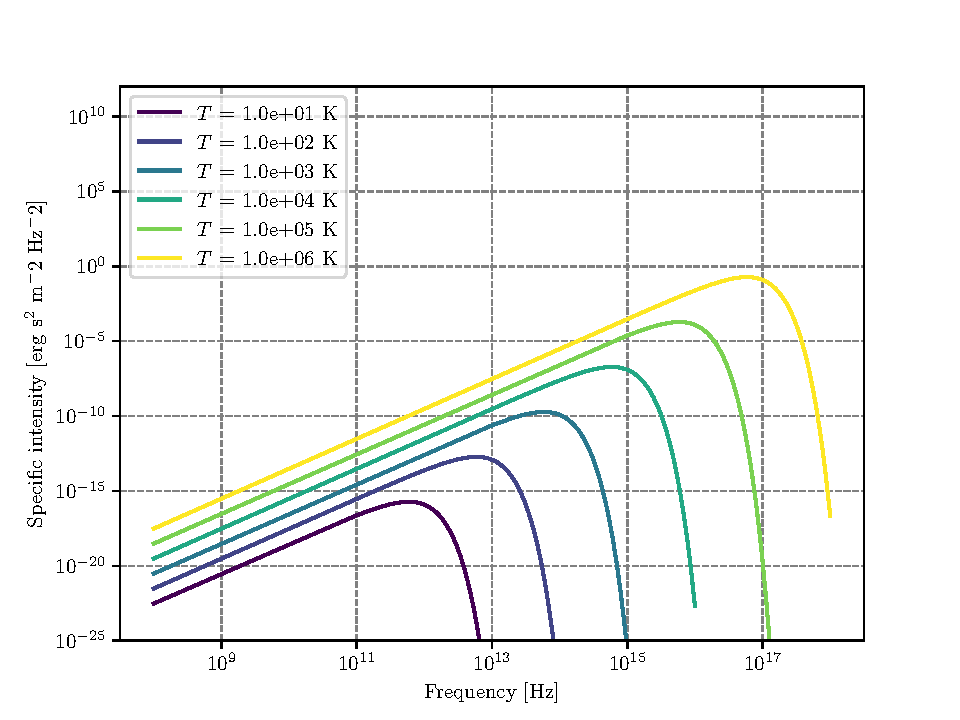
\includegraphics[width=0.9\textwidth]{img/blackbody.pdf}
	\caption{Blackbody frequency spectrum.}
    \label{fgr:planckfunction}
\end{figure}
\par It's important to notice that, in principle, such a fundamental result holds only in \emph{strict thermodynamic equilibrium} (STE), but it's possible to generalize this formulation for less "restrictive" environments.
\par An incredible number of important results descends from (\ref{eq:blackbodyintensity}), and it may be worthwhile to cite at least some of them, starting from Stefan-Boltzmann law. We'll use the following result without proving it 
\begin{equation*}
	\int_{0}^{+\infty} B_{\nu}(T)\,\text{d}\nu = \frac{2h}{c^{2}}\frac{\pi^{4}}{15}\left(\frac{kT}{h}\right)^{4}
\end{equation*}
\par Computing the bolometric flux and the bolometric energy density by integrating over all frequencies using what we've just written down, you find the following 
\begin{equation*}
	U(T) = aT^{4} \quad F(T) = \sigma_{SB}T^{4}
\end{equation*}
\par Clearly the two constants $a$ and $\sigma_{SB}$ cannot be independent, and are actually related by the integral we've previously calculated. Using for example\footnote{The emergent flux from an isotropically emitting surface (such as a blackbody) is $\pi\cdot \text{brightness}$ which is none other than the specific intensity.}
\begin{equation*}
	F(T) = \pi \int_{0}^{+\infty} B_{\nu}(T)\,\text{d}\nu
\end{equation*}
you can easily find out that the \emph{Stefan-Boltzmann constant} is equal to $$ \sigma_{SB} = \frac{2\pi^{5}k^{4}}{15c^{2}h^{3}}$$
and the relation with $a$ is simply $\sigma_{SB} = ac/4$.
\par The equation 
\begin{equation}
	F(T) = \frac{2\pi^{5}k^{4}}{15c^{2}h^{3}} T^{4}
	\label{eq:SB}
\end{equation}
is what is usually known as the \emph{Stefan-Boltzmann law}.
\par Let us now consider two different regimes for eq.\ref{eq:blackbodyintensity}: $h\nu/kT \ll 1$ and $h\nu/kT \gg 1$. The first yields what is commonly known as the Rayleigh-Jeans Law which is, sadly, pretty much relevant only for radioastronomy.
\par Since 
\begin{equation*}
	\exp\left(\frac{h\nu}{kT}\right) = 1+\frac{h\nu}{kT}+o\left(\frac{h\nu}{kT}\right)^{2}
\end{equation*} 
the blackbody radiation assumes the much simpler form of
\begin{equation*}
	B_{\nu}^{RJ} = \frac{2\nu^{2}}{c^{2}}kT
\end{equation*}
\par Another important results is achieved in the opposite regime, when the exponential term is rather larger than unity
\begin{equation*}
	B_{\nu}^{W} = \frac{2h\nu^{3}}{c^{2}}\exp\left(-\frac{h\nu}{kT}\right)
\end{equation*}
This expression is known as Wien's Law.
\subsection*{Characteristic Temperatures}
Starting from the blackbody spectrum we can give various definitions of temperature, that are going to be more and less useful when dealing with stars. The definitions are those of \cite{1986rpa..book.....R}.
\subsubsection*{Brightness Temperature}
One way of characterizing brightness (specific intensity) at a certain frequency is to give the temperature of the blackbody having the same brightness at that frequency. That is, for any value $I_{\nu}$ we define $T_{b}(\nu)$ by the relation
\begin{equation*}
    I_{\nu} = B_{\nu}(T_{b})   
\end{equation*}
this way of specifying brightness has the advantage of being closely connected with the physical properties of the emitter, and has the simple unit (K).
\par This procedure is used especially in radio astronomy, where the Rayleigh-Jeans law is usually applicable.
\begin{equation}
    T_{b} = \frac{c^{2}}{2\nu k}I_{\nu} \quad h\nu/kT \ll 1
\end{equation}
Note that the uniqueness of the definition of brightness temperature relies on the monotonicity property of Planck‘s law. Also note that, in general, the brightness temperature is a function of $\nu$.
\subsubsection*{Color Temperature}
Often a spectrum is measured to have a shape more or less of blackbody form, but not necessarily of the proper absolute value. For example, by measuring $F_{\nu}$, from an unresolved source we cannot find $I_{\nu}$, unless we know the distance to the source and its physical size.
\par By fitting the data to a blackbody curve without regard to vertical scale, a color temperature $T_{c}$, is obtained. Often the “fitting” procedure is nothing more than estimating the peak of the spectrum and applying Wien’s displacement law to find a temperature.
\subsubsection*{Effective Temperature}
The effective temperature of a source $T_{eff}$ is derived from the total amount of flux, integrated over all frequencies, radiated at the source. We obtain $T_{eff}$ by equating the actual flux $F$ to the flux of a blackbody at temperature $T_{eff}$
\begin{equation}
    F = \int I_{\nu}\cos\theta \,\text{d}\nu\,\text{d}\Omega := \sigma T_{eff}^{4}
    \label{eq:effectivetemperature} 
\end{equation}
\newpage
\section*{Appendix C: Christoffel Symbols}

\par For a symmetric, metric-compatible covariant derivative $\nabla_{\mu}$, the Christoffel symbols are given by
\begin{equation}
    \christoffel{\mu}{\nu}{\alpha} = \frac{1}{2}g^{\lambda\alpha}(\partial_{\mu}g_{\lambda\nu}+\partial_{\nu}g_{\mu\lambda}-\partial_{\lambda}g_{\mu\nu})
\end{equation}
\par For the FLWR metric (\ref{eq:FRW}), the Christoffel symbols are given by
\begin{align*}
    & \christoffel{1}{1}{0} = \frac{a\dot{a}}{1-kr^{2}} & \christoffel{1}{1}{1} = \frac{kr}{1-kr^{2}} \\
    & \christoffel{2}{2}{0} = a\dot{a}r^{2} & \christoffel{3}{3}{0} = a\dot{a}r^{2}\sin^{2}\theta \\
    & \christoffel{0}{j}{i} = \frac{\dot{a}}{a}\delta^{i}_{j}=H\delta^{i}_{j} & \christoffel{0}{1}{1} = \frac{\dot{a}}{a} = H \\
    & \christoffel{2}{2}{1} = -r(1-kr^{2}) &\christoffel{3}{3}{1} = -r(1-kr^{2})\sin^{2}\theta \\
    & \christoffel{1}{2}{2} = \christoffel{1}{3}{3} = \frac{1}{r} \quad & \christoffel{3}{3}{2} = -\sin\theta\cos\theta\\
    & \christoffel{2}{3}{3} = \cot\theta  & \christoffel{0}{0}{i} = 0\\
    & \christoffel{0}{0}{0} = 0 & \christoffel{i}{0}{0} = 0\\
\end{align*}
or related to this by symmetry. The non-zero components of the Ricci tensor are
\begin{align*}
    & R_{00} = -3\frac{\ddot{a}}{a} \\
    & R_{11} = \frac{a\ddot{a}+2\dot{a}^{2}+2k}{1-kr^{2}}\\
    & R_{22} = r^{2}(a\ddot{a}+2\dot{a}^{2}+2k)\\
    & R_{33} = r^{2}(a\ddot{a}+2\dot{a}^{2}+2k)\sin^{2}\theta
\end{align*}
and the Ricci scalar is then
\begin{equation*}
    R = 6\left[\frac{\ddot{a}}{a}\left(\frac{\dot{a}}{a}\right)^{2}+\frac{k}{a^{2}}\right]
\end{equation*}

\newpage

\section*{Appendix D: Where the D stands for Demonstration}

\subsection*{The FLRW Killing Tensor}

In Chapter \ref{ch:iv} we've defined at a certain point a Killing tensor (\ref{eq:killingtensor}) but I never showed that it actually satisfies Killing's equation. Our goal is to show that the tensor
\begin{equation}
    K_{\mu\nu} = a^{2}(g_{\mu\nu}+u_{\mu}u_{\nu})
\end{equation}
satisfies $\nabla_{(\sigma}K_{\mu\nu)} = 0$.
\par Let's start from observing that $K_{\mu\nu}$ is a spatial projector
\begin{equation}
    u^{\nu}K_{\mu\nu} = a^{2}(u^{\nu}g_{\mu\nu} + u_{\mu}u_{\nu}u^{\nu}) = 0
\end{equation}
since $u_{\nu}u^{\nu} = -1$. This means that we can define $h_{\mu\nu} = g_{\mu\nu}+u_{\mu\nu}$ so that $K_{\mu\nu} = a^{2}h_{\mu\nu}$. Note that $h_{\mu\nu}$ coincides with the spatial sections of the FLRW metric.
\par Before calculating the covariant derivative of the alleged Killing tensor, let's first check
\begin{align*}
    \nabla_{\mu}u_{\nu} &= \partial_{\mu}u_{\nu} - \christoffel{\mu}{\nu}{\lambda}u_{\lambda}\\
    &= +\christoffel{\mu}{\nu}{0} = \frac{1}{2}g^{00}\partial_{0}g_{\mu\nu}\\
    &= -\frac{1}{2}\partial_{0}(h_{\mu\nu}-u_{\mu}u_{\nu})\\
    &= -\frac{1}{2}\partial_{0}h_{\mu\nu} = -\frac{1}{2}\partial_{0}(a^{2}\tilde{h}_{\mu\nu}) = -a\dot{a}\tilde{h}_{\mu\nu} = -Hh_{\mu\nu}
\end{align*}
We can now expand the covariant derivative of $K_{\mu\nu}$
\begin{align*}
    \nabla_{\lambda}K_{\mu\nu} &= h_{\mu\nu}\nabla_{\lambda}a^{2}+a^{2}\nabla_{\lambda}h_{\mu\nu}\\
    &= 2a\dot{a}u_{\lambda}h_{\mu\nu} + a^{2}\nabla_{\lambda}h_{\mu\nu}\\
    &= 2a\dot{a}u_{\lambda}h_{\mu\nu} + a^{2}(u_{\mu\nabla_{\lambda}u_{\nu}}+u_{\nu}\nabla_{\lambda}u_{\mu})
\end{align*}
where we can now substitute $\nabla_{\mu}u_{\nu} = -Hh_{\mu\nu}$ to obtain
\begin{align*}
    \nabla_{\lambda}K_{\mu\nu} &= 2a\dot{a}u_{\lambda}h_{\mu\nu} -a\dot{a}(u_{\mu}h_{\nu\lambda}+u_{\nu}h_{\mu\lambda})\\
    &= a\dot{a}\left[(u_{\lambda}h_{\mu\nu}-u_{\mu}h_{\lambda\nu})+(u_{\lambda}h_{\mu\nu}-u_{\nu}h_{\lambda\mu})\right]\\
    &= 2a\dot{a}\left[u_{[\lambda}h_{\mu]\nu} +u_{[\lambda}h_{\nu]\mu} \right]
\end{align*}
\par At this point, we can easily see that the symmetrization $\nabla_{(\sigma}K_{\mu\nu)}$ of the previous expression yields zero, thus proving that $K_{\mu\nu}$ is indeed a Killing tensor.

\subsection*{Geodesics on a perturbed FLRW metric}

In Chapter \ref{ch:v} we presented the gauge-invariant version of the conformal, perturbed FLRW metric 
\begin{equation}
    \diff{s^{2}} = a^{2}(\eta)\left[-(1+2\psi)\diff{\eta^{2}} + (1-2\phi)\delta_{ij}\diff{x^{i}}\diff{x^{j}}\right]
    \label{eq:gauge-inv-fix-FLRW}
\end{equation}
and obtained from there the geodesic equation and the resulting equation for the evolution of the photon energy in conformal time, which was crucial to obtain the CMB power spectrum. It is the purpose of this subsection to prove the result we have obtained (\ref{eq:cmbgeodesics}).
\par First, you can easily compute the relevant Christoffel's symbols (the ones with a 0-upper index)
\begin{equation}
    \christoffel{0}{0}{0} = \mathcal{H} + \frac{\psi'}{1+2\psi} \quad \christoffel{0}{i}{0} = \frac{\partial_{i}}{1+2\psi} \quad \christoffel{i}{j}{0} = \frac{1}{1+2\psi}\left[\mathcal{H}(1-2\phi)-\phi'\right]\delta_{ij}
\end{equation}
Please note that we're working with coordinates $(\eta, x_{1}, x_{2}, x_{3})$, and that with the prime superscript we're referring to conformal-time (partial) derivatives.
\par The geodesic equation is thus 
\begin{equation}
    \small{
    \der{p^{0}}{\lambda} = -\left(\mathcal{H} + \frac{\psi'}{1+2\psi}\right)(p^{0})^{2}-2\frac{\partial_{i}}{1+2\psi}p^{0}p^{i}-\frac{1}{1+2\psi}\left[\mathcal{H}(1-2\phi)-\phi'\right]\delta_{ij}p^{i}p^{j}
    }
\end{equation}
Now let's exploit the null-condition for photons 
\begin{equation}
    p_{\mu}p^{\mu} = g_{\mu\nu}p^{\mu}p^{\nu} = g_{00}(p^{0})^{2}+g_{ij}p^{i}p^{j}
\end{equation}
which after substituting the relevant components of the metric turns into 
\begin{equation}
    \delta_{ij}p^{i}p^{j} = \frac{1+2\psi}{1-2\phi}(p^{0})^{2}
\end{equation}
which we can use to write the spatial component of the momentum as 
\begin{equation}
    p^{i} = \sqrt{\frac{1+2\psi}{1-2\phi}}p^{0}\hat{p}^{i}
\end{equation}
This means that the geodesic equation is now
\begin{equation}
    \small{
    \frac{1}{(p^{0})^{2}}\der{p^{0}}{\lambda} = -\left(\mathcal{H} + \frac{\psi'}{1+2\psi}\right)-2\frac{\partial_{i}\psi}{1+2\psi}\sqrt{\frac{1+2\psi}{1-2\phi}}\hat{p}^{i}-\frac{1}{1-2\phi}\left[\mathcal{H}(1-2\phi)-\phi'\right]
    }
\end{equation}
But since 
\begin{equation}
    p^{\mu} = \der{x^{\mu}}{\lambda} \implies p^{0} = \der{\eta}{\lambda}
\end{equation}
hence
\begin{equation}
    \small{
    \frac{1}{p^{0}}\der{p^{0}}{\eta} = -\left(\mathcal{H} + \frac{\psi'}{1+2\psi}\right)-2\frac{\partial_{i}\psi}{1+2\psi}\sqrt{\frac{1+2\psi}{1-2\phi}}\hat{p}^{i}-\frac{1}{1-2\phi}\left[\mathcal{H}(1-2\phi)-\phi'\right]
    }
\end{equation}
The energy of the photon as measured along a geodesic from a comoving observer is just $E_{\gamma} = -u_{\mu}p^{\mu}$, where $u_{\mu}u^{\mu} = -1$. Expanding and choosing the negative sign\footnote{The choice of the sign was made so that to a positive $p^{0}$ corresponded a positive $E_{\gamma}$.} for $u_{0}$ we get 
\begin{equation}
    u_{0} = -a\sqrt{1+2\psi}
\end{equation}
and thus 
\begin{equation}
    E_{\gamma} = a\sqrt{1+2\psi}p^{0}
\end{equation}
We can take the logarithmic derivative of last equation to find
\begin{equation}
    \frac{1}{E_{\gamma}}\der{E_{\gamma}}{\eta} = \mathcal{H} + \frac{1}{p^{0}}\der{p^{0}}{\eta}+\frac{1}{1+2\psi}\der{\psi}{\eta}
\end{equation}
Substituting into the expanded geodesic equation we conclude
\begin{equation}
    \boxed{
        \frac{1}{E_{\gamma}}\der{E_{\gamma}}{\eta} = - \mathcal{H}+\frac{1}{1+2\psi}(\hat{p}^{i}\partial_{i})\psi\left[1-2\sqrt{\frac{1+2\psi}{1-2\phi}}\right] + \frac{\phi'}{1-2\phi}
    }
    \label{eq:energy-perturbedflrw}
\end{equation}
where we have exploited the chain-rule for the total derivative
\begin{equation}
    \der{\psi}{\eta} = \parder{\psi}{\eta} + \parder{x^{i}}{\eta}\partial_{i}\psi
\end{equation}
In principle, this last equation holds exactly, but we can exploit the underlying assumption that $\psi,\,\phi \ll 1$ (so that they are proper perturbations) and Taylor-expand (\ref{eq:energy-perturbedflrw}), neglecting second order terms. What we obtain is
\begin{equation}
    \frac{\phi'}{1-2\phi} \approx \phi' \quad \frac{1}{1+2\psi}\left[1-2\sqrt{\frac{1+2\psi}{1-2\phi}}\right] \approx -1 +\frac{2\phi}{1+2\psi} \approx 1
\end{equation}
and so we obtain 
\begin{equation}
    \frac{1}{E_{\gamma}}\der{E_{\gamma}}{\eta} = - \mathcal{H}-(\hat{p}^{i}\partial_{i})\psi + \phi'
\end{equation}
which is exactly the expression we've found in Chapter \ref{ch:v}.
